%\documentclass[runningheads]{llncs}
\documentclass{llncs}
%\usepackage{graphicx}
\usepackage{xcolor}
\usepackage{amssymb}
\usepackage{dsfont}
\usepackage{amsmath} 

\usepackage{url}
\usepackage{cancel}
\usepackage{verbatim}
\usepackage{alltt}
\usepackage{graphicx}
\usepackage{prooftree}

\usepackage{latexsym}
\usepackage{xspace}
%\usepackage{draft} REVOIR
\usepackage{comment}
%\usepackage{ntheorem}
%\usepackage{amsthm} % \proof seems to exist in llncs

\newcommand{\revoir}[1]{\mbox{{[*** {\bfseries\large #1} ***]}}}
\newcommand{\nouveau}[1]{\textcolor{blue}{#1}}

\newcommand{\egdef}%
   {\ensuremath{\:\mathrel{\raisebox{-.7ex}%
   {$\stackrel{\rm def}{=\mkern-8mu=}$}}\:}}

\newcommand{\simlight}{\texttt{simlight}\xspace}

\newtheorem{Prog}{Program}
%\newcommand{\idcoq}[1]{\texttt{#1}}
\newcommand{\idcoq}[1]{\ensuremath{\mathit{#1}}}
\newcommand{\impl}{\ensuremath{\Rightarrow}}
\newcommand{\flequiv}{\ensuremath{\leftrightarrow}}
\newcommand{\todo}[1]{\textcolor{blue}{\textsc{[#1]}}}
\newcommand{\XM}[1]{{\color{red} #1}} % Xiaomu's editing
\newcommand{\JFM}[1]{{\color{red} #1}} % JF's editing

% BEGIN For coqdoc 

\newenvironment{coqdoccode}{}{}

\newlength{\coqdocbaseindent}
\setlength{\coqdocbaseindent}{0em}

\newcommand{\coqdef}[3]{#3}
\newcommand{\coqref}[2]{#2}
\newcommand{\coqexternalref}[3]{#3}

% Beginning of a line without any Coq indentation
\newcommand{\coqdocnoindent}{\noindent\kern\coqdocbaseindent}
% Beginning of a line with a given Coq indentation
\newcommand{\coqdocindent}[1]{\noindent\kern\coqdocbaseindent\noindent\kern#1}
% End-of-the-line
\newcommand{\coqdoceol}{\hspace*{\fill}\setlength\parskip{0pt}\par}
% Empty lines (in code only)
\newcommand{\coqdocemptyline}{\vskip 0.4em plus 0.1em minus 0.1em}

% own name
\newcommand{\coqdoc}{\textsf{coqdoc}}

% pretty underscores (the package fontenc causes ugly underscores)
%BEGIN LATEX
\def\_{\kern.08em\vbox{\hrule width.35em height.6pt}\kern.08em}
%END LATEX

% macro for typesetting keywords
\newcommand{\coqdockw}[1]{\texttt{#1}}

% macro for typesetting variable identifiers
\newcommand{\coqdocvar}[1]{\textit{#1}}

% macro for typesetting constant identifiers
\newcommand{\coqdoccst}[1]{\textsf{#1}}

% macro for typesetting module identifiers
\newcommand{\coqdocmod}[1]{\textsc{\textsf{#1}}}

% macro for typesetting module constant identifiers (e.g. Parameters in
% module types)
\newcommand{\coqdocax}[1]{\textsl{\textsf{#1}}}

% macro for typesetting inductive type identifiers
\newcommand{\coqdocind}[1]{\textbf{\textsf{#1}}}

% macro for typesetting constructor identifiers
\newcommand{\coqdocconstr}[1]{\textsf{#1}}

% macro for typesetting tactic identifiers
\newcommand{\coqdoctac}[1]{\texttt{#1}}

% These are the real macros used by coqdoc, their typesetting is 
% based on the above macros by default.

\newcommand{\coqdoclibrary}[1]{\coqdoccst{#1}}
\newcommand{\coqdocinductive}[1]{\coqdocind{#1}}
\newcommand{\coqdocdefinition}[1]{\coqdoccst{#1}}
\newcommand{\coqdocvariable}[1]{\coqdocvar{#1}}
\newcommand{\coqdocconstructor}[1]{\coqdocconstr{#1}}
\newcommand{\coqdoclemma}[1]{\coqdoccst{#1}}
\newcommand{\coqdocclass}[1]{\coqdocind{#1}}
\newcommand{\coqdocinstance}[1]{\coqdoccst{#1}}
\newcommand{\coqdocmethod}[1]{\coqdoccst{#1}}
\newcommand{\coqdocabbreviation}[1]{\coqdoccst{#1}}
\newcommand{\coqdocrecord}[1]{\coqdocind{#1}}
\newcommand{\coqdocprojection}[1]{\coqdoccst{#1}}
\newcommand{\coqdocnotation}[1]{\coqdockw{#1}}
\newcommand{\coqdocsection}[1]{\coqdoccst{#1}}
\newcommand{\coqdocaxiom}[1]{\coqdocax{#1}}
\newcommand{\coqdocmodule}[1]{\coqdocmod{#1}}

% END For coqdoc 

% macros for this paper
\newcommand{\diag}{\coqdocvar{diag}\xspace}
\newcommand{\inversion}{\coqdoctac{inversion}\xspace}
\newcommand{\inv}{\coqdoctac{inv}\xspace}
\newcommand{\casetac}{\coqdoctac{case}\xspace}
\newcommand{\match}{\coqdoctac{match}\xspace}
\newcommand{\with}{\coqdoctac{with}\xspace}
\newcommand{\intac}{\coqdoctac{in}\xspace}
\newcommand{\retac}{\coqdoctac{return}\xspace}
\newcommand{\refine}{\coqdoctac{refine}\xspace}
\newcommand{\Prop}{\coqdockw{Prop}\xspace}
\newcommand{\True}{\coqdocvar{True}\xspace}
\newcommand{\eveni}{\coqdocvar{even\_i}\xspace}
\newcommand{\EZ}{\coqdocvar{E0}\xspace}
\newcommand{\ET}{\coqdocvar{E2}\xspace}
\newcommand{\evenf}{\coqdocvar{even\_f}\xspace}
\newcommand{\prone}{\coqdocvar{pr\_1}\xspace}
\newcommand{\prET}{\coqdocvar{premises\_E2}\xspace}
\newcommand{\EXPR}{\coqdocvar{EXPR}\xspace}
\newcommand{\PROOFEV}{\coqdocvar{PROOF\_EV}\xspace}
\renewcommand{\PROOFEV}{\mathit{PE}}

% For automated inclusion of .tex files generated from coqdoc
\newcommand{\coqdocinput}[1]{\input{#1}}

\newcommand{\union}{\ensuremath{\cup}}

\newenvironment{ml}
  {\begin{alltt}
   \footnotesize} %% 3.12.0
  {\end{alltt}
  }

\newenvironment{coq}
  {\begin{alltt}
   \footnotesize} %% 8.3pl2 (April 2011)
  {\end{alltt}
  }

\newenvironment{humC}
  {\begin{alltt}
   \footnotesize}
  {\end{alltt}
  }



\begin{document}

\title{Scaling up Small Inversions
}
\titlerunning{Scaling up Small Inversions}
% Official order as registered at CPP
\author{Jean-Fran\c{c}ois Monin\inst{1,2}
\and 
Xiaomu Shi\inst{1}
}
\institute{%
Universit\'{e} de Grenoble 1 - LIAMA
\and CNRS - LIAMA
}
\authorrunning{J.-F. Monin, X. Shi}

\maketitle

\begin{abstract}
  When reasoning on formulas involving large-size inductively defined
  relations, such as the semantics of a real programming language,
  many steps require the inversion of a hypothesis. The built-in
  ``inversion'' tactic of Coq can then be used, but it suffers from
  severe controllability and efficiency issues.  A proof-trick called
  small inversions by one of the co-authors provides a part of the
  solution. It is based on a suitable auxiliary diagonal
  predicate. However, many important practical situations are not
  covered by this technique.  We present here an improvement inspired
  by the impredicative encoding of inductive data-structures. Our
  experiments in the SimSoC-Cert project show that this technique
  successfully scales up to proofs of non-trivial programs according
  to the operational semantics of C as defined in Compcert.
\end{abstract}



%-------------------------------------------------------------------------
\section{Introduction}
\label{sec:intro}

Type-theoretic settings such as Coq \cite{CoqManualV83,BC04,cpdt}
offer two elementary ways of constructing new objects:
functions and inductive types\footnote{%
Co-inductive types are available as well. 
However, this paper does not depend on issues related to finiteness
of computations:
what is said about inductive types holds as well for co-inductive types.
}. 
%\todo{Inductive are used for datatypes and relations, fixpoints for functions.}
%
For instance, even on Peano natural numbers can be inductively characterized 
by the following two rules:

\[
\begin{prooftree}
\using {\coqdocvar{E0}}
\justifies\coqdocvar{even\_i}~ 0
\end{prooftree}
\qquad
\begin{prooftree}
\coqdocvar{even\_i}~ n
\using {\coqdocvar{E2}}
\justifies\coqdocvar{even\_i (S (S n))}
\end{prooftree}
\]


%\coqdocinput{chunk1}

\noindent
%%Rule names such as \coqdocvar{E1} and \coqdocvar{E2}
Rules E1 and E2
serve as canonical justifications for \coqdocvar{even\_i}, 
they are called the \emph{constructors} of the inductive definition.

Now, assume a hypothesis $H$ claiming
that \coqdocvar{even\_i (S (S (S x)))} for some natural number $x$.
Then, by looking at the definition of \coqdocvar{even\_i}, 
we see that only \coqdocvar{E2} could justify $H$,
and we can conclude that \coqdocvar{even\_i (S x)}.
Similarly,  \coqdocvar{even\_i} 1 can be considered as an
absurd hypothesis, since \coqdocvar{(S 0)} matches neither
0 nor \coqdocvar{(S (S n))}, 
none of the two possible canonical ways of proving \coqdocvar{even\_i},
namely \coqdocvar{E0} and \coqdocvar{E2} can be used.
Such proof steps are called \emph{inversions},
because they use justifications such as \coqdocvar{E0} and \coqdocvar{E2}
in the opposite way, i.e.,
from their conclusion to their premises. 
Note that \coqdocvar{even\_i} 3, \coqdocvar{even\_i} 5, etc. 
%do not immediately yield the absurd by inversion.
do not immediately yield the contradiction by inversion.
However, by iterating the first inversion step, we eventually get
\coqdocvar{even\_i} 1 and then the desired result using a last inversion.
This illustrates that inversion is closer to case analysis than to induction.

Indeed, as we will see below, 
inversion can be decomposed into elementary proof steps,
where the key step is a primitive case analysis on the considered
inductive object (the hypothesis $H$, in our previous example). 
However, this decomposition is very often far from trivial because,
in the general case, rules may include several premises,
premises and conclusions may have several arguments and
some of these arguments can be shared.
Still, inversion turns out to be extremely useful in practice.
Well-known instances are related to programming languages,
because whose semantics is described using complex inductively defined
relations. 

Note that it may be worth considering a (recursive) \emph{function}
for defining a predicate, rather than an inductive relation.
For instance, in Coq syntax, an alternative way to specify even
numbers is as follows:

% Now, assume a goal containing a hypothesis $H$ claiming
% that \coqdocvar{even\_i (S x)} for some natural number $x$.
% Then, by looking at the definition of \coqdocvar{even\_i}, 
% we can conclude that $x$ is \coqdocvar{(S y)}
% for some $y$ satisfying \coqdocvar{even\_i y}.

\medskip
\coqdocinput{chunk11}
\medskip

\noindent
Here \coqdocvar{True} denotes the trivially provable proposition,
and \coqdocvar{False} denotes the absurd proposition.
%
Using \coqdocvar{even\_f} is much simpler in the previous situations:
for instance, \coqdocvar{even\_f (S (S (S x)))} just \emph{reduces} to
\coqdocvar{even\_f (S x)} using computation.
In other words, computation provides inversion for free.
Therefore, one may wonder why we should bother with inductively defined
relations.
Two kinds of answers can be given.

One of them is that an inductive definition allows us 
to focus exactly on the relevant values
whereas, with functional definitions,
we have to deal with the full domain,
which can be much bigger in general.
In our example above,
suppose that we want to prove a statement such as
$\forall n, \mathit{even}\:n \impl P\: n$.
We can always attempt an induction on $n$,
but this strategy enforces to reason on all numbers, 
including odd numbers.
%If even is encoded with even_f,
If $\mathit{even}$ is the recursive function above \coqdocvar{even\_f},
%this is no other option.
there is no other option.
However, using \coqdocvar{even\_i}, 
we have the additional opportunity to make an induction on 
(the shape of) $\coqdocvar{even\_i}\;n$,
without needing to bother about odd numbers.

Another issue is that it is not always convenient or even possible to
provide a functional definition of a predicate.
Whenever possible,
an $n$-ary relation $R$ on $A_1 \times \ldots A_n$, % with $n \ge 2$,
is advantageously modeled by a function from $A_1, \ldots A_{n-1}$ to $A_n$.
But it requires $R$ to be functional (deterministic) and moreover,
in type-theoretical settings such as CIC, to be total.
If the relation is non-deterministic,
we still can try to 
define it by a function returning either \coqdocvar{True}
or \coqdocvar{False}, as is the case for \coqdocvar{even\_f};
this essentially amounts to provide a decision procedure for 
the intended predicate\footnote{
Note that a 1-ary relation $P$ on $A_1$ is isomorphic to a 
binary relation on $\mathbf{1}\times A_1$,
where $\mathbf{1}$ is a type with exactly one inhabitant.
If $P$ holds for at least two values on $A_1$, 
it can be clearly considered as a non-deterministic 
function from $\mathbf{1}$ to $A_1$.
}.
This is not always possible and, even if we can find such an
algorithm, it may be hindered by undesired encoding tricks,
which will induce additional complications in proofs. 
Moreover, a requirement of formal methods expresses that
high-level definitions and statements should be as clear 
as possible in order to be convincing. 
The inductive style is not always better than the functional
style, but it is often enough the case so that we cannot
ignore it. 
For technical reasons, it is sometimes worth to consider
a functional version and an inductive version of the same notion.
Even if the functional version is much better at inversion-like
proof steps, 
the two versions have to be proved equivalent and there,
the need for inverting the inductive version almost inevitably shows up.


All these considerations are especially relevant in the case
of the operational semantics of programming languages,
either in small-step or in big-step style \cite{nielson}. 
Such semantics define transitions between states,
language constructs and,
very often, additional arguments such as input/output events. 
They may be inductively defined, 
with at least one rule for each language construct. 
A tutorial example of a toy (but Turing-complete) language 
formally defined in Coq along these lines
is given in \cite{Pierce:SF}
and routinely used as a teaching support in many universities.
A much more involved example
is the semantics of a fairly large subset of C, as defined in 
the Compcert project \cite{Leroy-Compcert-CACM}.

In the SimSoC-cert project \cite{cpp11}, 
we use this semantics to perform proofs of 
an instruction set simulator for ARM,
which is at the heart of SimSoC~\cite{rapido11}, 
a simulator of embedded systems written in C and C++.
Many inversions are needed in our proofs.

\medskip
The practical need for automating inversion has been identified
many years ago.
The first implementations for Coq and LEGO
are analyzed and explained in
\cite{cornes95automating} for Coq
and \cite{McBride96} for LEGO.
Since then, the main tool available to the Coq user is
a tactic called \inversion which,
basically performs a case analysis over a given hypothesis
according to its specific specific arguments,
removes absurd cases,
introduces relevant premises in the environment
and performs suitable substitutions in the whole goal.
%
This tactic works remarkably well,
%though it fails in seldom intricate cases,
though it fails in rare intricate cases,
as reported in mailing lists. 
%
However, the price to pay for its generality
is a high complexity of the formal proof-term underlying
an inversion. 
Does it reflect an unnecessarily complex formalization of a 
(at first sight) rather simple idea?
Anyway, 
beyond slowing down the evaluation of scripts which make
an intensive use of this tactic, 
a practical consequence is that
unpleasantly heavy proof terms can unexpectedly occur in
functions defined in interactive mode.

More importantly, in our opinion, using this tactic
introduces many new hypotheses in the environment.
Their names are automatically generated
and a sequel of the script depends on them.
Moreover such introduced hypotheses could be inverted again,
and so on.
This poses a problem of robustness which is very serious
in large developments:
updating the inductive relation or
even minor modifications in another part of the development
may result in a complete renaming 
inside a proof script,
which has then to be debugged line by line.
%The situation is better in recent version of Coq, 
%since \inversion can optionally be given the names of all hypotheses
%to be introduced.
The situation is better when using \inversion with variant in order to
give names to all introduced hypotheses.
Still, their number and contents is hard to predict,
%which makes \inversion hardly usable in high-level tactics.
which makes \inversion hardly usable in high-level tactics who intent to
invoke \inversion results.

In \cite{small_inv}, 
the first author introduced a technique 
for performing
so-called \emph{small inversions}. 
This technique is rather flexible and is available in several variants.
Our goal was to demystify the magics behind \inversion
and to propose a practical hand-crafted alternative
to this tactic, 
providing much smaller proof terms as well as
a full control of the user on the behavior of inversion.
The idea was illustrated only on very simple examples
and had to be validated on realistic applications. 

We report here such an experiment, 
in the framework of the SimSoC-cert project introduced above.
It turned out that significant changes had to
be made in order to make the initial idea able
to scale up.
%
The contributions presented here are then:
\begin{itemize}
\item an improvement of the main variant from \cite{small_inv},
  which makes 
  it both simpler to use and more powerful;
\item its illustration on a significant application,
  which involves an intensive use of inversions on 
  big inductive relations coming from the Compcert project.
\end{itemize}

The concrete setting considered here is the Coq proof assistant,
but the technique can be adapted to any proof assistant based
on the Calculus of Inductive constructions or a similar type theory, 
such as LEGO, Matita. %or Agda.
The rest of the paper is organized as follows.
Section~\ref{sec:absurd}
recalls the principle of small inversions as introduced in \cite{small_inv}.
Section~\ref{sec:improvement} then explains its limitations
and how to overcome them,
while Section~\ref{sec:simsoccert} contains a summary
of the application to SimSoC-cert.
We conclude in Section~\ref{sec:conclusion} with a comment
on our achievements and some perspectives.




%%% Local Variables: 
%%% mode: latex
%%% TeX-master: "cpp12"
%%% End: 

\svnidlong
{$HeadURL: svn+ssh://blanqui@scm.gforge.inria.fr/svnroot/simsoc-cert/papers/itp13/sminv-absurd.tex $}
{$LastChangedDate: 2013-04-18 13:09:21 +0200 (jeu. 18 avril 2013) $}
{$LastChangedRevision: 2302 $}
{$LastChangedBy: monin $}

% Author: \svnfileauthor; Revision: \svnfilerev; Last changed on: \svnfiledate; 
% URL: \url{\svnkw{HeadURL}}

\begin{thoughts}
\itshape
\hfil -----------------------------------------------------------------------------------\par
\hfil \textbf{Changes on \currfilename}

Author: \svnfileauthor; Revision: \svnfilerev; Last changed on: \svnfiledate
\end{thoughts}

% svn propset svn:keywords 'LastChangedBy LastChangedRevision LastChangedDate HeadURL' thisfile.tex

%%%%%%%%%%%%%%%%%%%%%%%%%%%%%%%%%%%%%%%%%%%%%%%%%%%%%%%%%%%%%%%%%%%%%%%%%%%%%
\section{A Handcrafted Inversion}
\label{sec:hci}

As noticed above, the heart of inversion is a suitable
pattern matching on the hypothesis to be analyzed.
With dependent types, it is possible for different branches
to return a result whose type depends on the constructor.
We make a systematic use of this feature:
our key ingredient is a diagonalization function $\diag$,
which will be used for specifying the type returned on each branch.
The exact shape of $\diag$ range from very simple to somewhat elaborated
according to the goal at hand. 

We recall the basics on dependent pattern matching,
then we successively consider three situations,
corresponding to increasingly complex variants of $\diag$.
In the two first situations, 
we consider inductive predicates with exactly one argument, for simplicity.
The first situation is when all cases are absurd.
The second is when a case is successful (or several cases)
and we need to extract the information contained in successful cases,
making new hypotheses in the environment.
Then we show how to deal with additional arguments,
so that constraints coming from the conclusion have to be propagated
on the new hypotheses.
Finally, we consider more elaborate dependent types
and show how our technique works on a case where \inversion fails.

\subsection{Dependent Pattern Matching}
\label{sec:dpm}

To start with, 
let us take again the example of even numbers.
Here is the corresponding Coq inductive definition.

\medskip
\coqdocinput{chunk21}
\medskip

\noindent
We see that each rule is given by a constructor in a dependent data type
-- also called an inductive predicate or relation because its sort is \Prop.
Therefore, the elementary way to decompose an object of type \eveni $n$
is to use dependent pattern matching.
This is already done by primitive tactics of Coq
such as \coqdockw{case} and \coqdockw{destruct},
which turn out to be powerful enough in many situations, 
when a condition is satisfied:
the conclusion of the current goal fits all arguments of 
the hypothesis to be analyzed by pattern matching.

Let us first illustrate 
dependent pattern matching on even numbers.
Consider a proof $\PROOFEV$ of type $\eveni\;n$
for some natural number $n$.
For each possible constructor, \EZ or \ET, 
we provide a proof term,
respectively $t_\EZ$ and $t_\ET$.
As usual, this term may depend on the arguments 
of the corresponding constructor,
none for \EZ and, say $x$ and $ex$ for \ET.
More importantly for us, $t_\EZ$ and $t_\ET$ may have
different \emph{types}:
the type $P\;n$ of the whole expression depends on $n$;
in the first branch, the type of $t_\EZ$ is $P\;0$ and
in the second branch, the type of $t_\ET$ is $P\; (S\: (S\:x))$.
Therefore, the syntax of the \coqdockw{match} construct
contains a \coqdockw{return} clause with the expected type
of the result $P\;n$ as an argument;
moreover, 
there is also an \coqdockw{in} clause for the type of $\PROOFEV$
which binds $n$:

%\smallskip
\coqdocinput{chunk22}
%\smallskip

\vspace*{-.7\baselineskip}
\noindent
Most of the time, Coq users do not need to go to this
level of detail: 
in interactive proof mode, 
if $n$ and $P\;n$ are clear from the context,
\casetac $\PROOFEV$ will do the job.
More precisely, if we have an hypothesis $H$ of type $\eveni\;n$
and a desired conclusion of type $P\;n$, 
\casetac $H$ will construct a proof term having the previous
shape and answer with two new subgoals:
one for $P\;0$ and one for $P\; (S\: (S\:x))$,
with $\eveni\;x$ as an additional assumption.

As a last remark, let us recall that
an inductive type may have two kinds of arguments.
We don't care about arguments which are ``fixed'' for all constructors:
they are not even considered in pattern matching.
In Coq they are called \emph{parameters}.
The other arguments are called \emph{indexes}.
For example, $\eveni$ has one index and no parameter.

\subsection{Auxiliary Diagonalization Function}
\label{sec:absurd}

More work is needed precisely when there is no obvious relationship
between the conclusion and the hypothesis to be analyzed.
This happens in particular when $H$ is absurd:
the goal should be discharged whatever is its conclusion.
This situation is covered as follows:
the conclusion is converted 
to an expression \diag $V$,
where $V$ is a value coming from $H$ 
and \diag a suitable diagonal function, such that
the dependent case analysis on $H$ provides only trivial subgoals.
For example, assume that we want to conclude
$4=7$ from the hypothesis $H: \eveni\;1$.
Our diagonal function is then defined as follows.

\medskip
\coqdocinput{chunk24}
%\smallskip

\noindent
Then the conclusion is converted to $\diag\;1$,
and the case analysis on $H$ 
automatically provides two subgoals $\diag\;0$
and $\diag\;(S\: (S\:y))$ for an arbitrary even natural number $y$.
Each of these goals reduce to \True, 
and we are done.
The proof term behind this reasoning is very short
($I$ is the standard proof of \True):

\medskip
\coqdocinput{chunk25}
%\smallskip

%\vspace*{-1.0\baselineskip}
Such functions were already introduced in~\cite{small_inv},
but they work well only for handling absurd hypotheses.
For instance, the examples presented below are out of reach
of~\cite{small_inv}.
In order to explain how to extract information from satisfiable hypotheses,
we start with an obvious generalization of the previous function
for inverting absurd hypotheses.

% \medskip
% \coqdocinput{chunk23}
% \medskip


%%% Local Variables: 
%%% mode: latex
%%% TeX-master: "itp13"
%%% End:

\svnidlong
{$HeadURL$}
{$LastChangedDate$}
{$LastChangedRevision$}
{$LastChangedBy$}

% Author: \svnfileauthor; Revision: \svnfilerev; Last changed on: \svnfiledate; 
% URL: \url{\svnkw{HeadURL}}

\begin{thoughts}
\itshape
\hfil -----------------------------------------------------------------------------------\par
\hfil \textbf{Changes on \currfilename}

Author: \svnfileauthor; Revision: \svnfilerev; Last changed on: \svnfiledate
\end{thoughts}

% svn propset svn:keywords 'LastChangedBy LastChangedRevision LastChangedDate HeadURL' thisfile.tex

%%%%%%%%%%%%%%%%%%%%%%%%%%%%%%%%%%%%%%%%%%%%%%%%%%%%%%%%%%%%%%%%%%%%%%%%%%%%%
\subsection{Handling Successful Cases}
\label{sec:improvement}


%\vspace*{-.7\baselineskip}
% Let us now consider what happens if $H$ is 
% $\eveni\;3$ instead of $\eveni\;1$. 
% As mentioned in the introduction, 
% a first inversion on $H$ will push $\eveni\;1$ in the environment, 
% and then we are back to the previous situation.
% In \cite{small_inv} we show that in such situations 
% the goal can be proved in a different way, by keeping
% the same diagonal function in the whole process.
% Here the conclusion is convertible to $\diag\;3$ with:

% \coqdocinput{chunk26}

% \vspace*{-.7\baselineskip}
% \noindent
% Then the case analysis on $H$ leaves a subgoal for \ET,
% since 3 matches $(S\: (S\:n))$.
% That is, we have to prove 
% $\diag\;(S\: (S\:y))$ with an additional hypothesis $Hy: \eveni\;y$.
% A case analysis on $Hy$ yields two subgoals:
% $\diag\;2$ and $\diag\;(S\: (S\: (S\: (S\:z))))$,
% because $y$ is either $0$ or $(S\: (S\:z))$, and
% these 2 subgoals reduce to \True.

% This strategy works for arbitrary large odd values,
% see \cite{small_inv} for more complex examples.
% Measurements on the corresponding proof terms showed
% that their size is 1 to 2 orders of magnitude smaller
% than with the standard \inversion of Coq.

% However, 
% the technique explained in the previous subsection 
% has to be extended in order to cover more general
% situations. 

A first easy improvement makes \diag independent
from the conclusion.
To this effect, we replace it with $(\forall X, X)$ 
in the first branch of \diag.
In our previous example, this yields

\vspace*{.5\baselineskip}

\coqdocinput{chunk27}

\noindent
Then the previous proof term 
(\match $H$ \intac $\eveni\;n$ \retac $\diag\;n$ \with 1 $\ldots$)
has the type $\forall X, X$
and then can be successfully applied to any current conclusion.
Alternatively, we can define a general function as follows:

%\vspace*{.5\baselineskip}

\smallskip
\coqdocinput{chunk29}


\medskip\noindent
Next consider the following theorem:

\smallskip
\coqdocinput{chunk28}
\smallskip

\noindent
The proof is by induction on $\eveni\;n$.
In the inductive step, we have to prove $\eveni\;m$
from the induction hypothesis $\eveni\:(n + m) \rightarrow \eveni\;m$
and a new hypothesis $H: \eveni\: (S\: (S\: (n + m)))$.
Intuitively, we want to invert $H$ in order to push $\eveni\:(n + m)$
in the environment. 
% The trick given at the end of Section~\ref{sec:absurd}
% is then of no help.
We can then adapt \prone as follows:

\smallskip
\coqdocinput{chunk30}

\noindent
Then, applying \prET to $H$ yields a function in continuation passing style.
Its type parameter $X$ is automatically identified to the conclusion
$\eveni\;m$, while $y$ is bound to $n+m$,
so that we get a new goal $\eveni\:(n+m) \rightarrow \eveni\;m$.
That is, we have exactly the expected inversion.
Functions such as \prone and \prET can be seen as inversion
lemmas, but note that their type is the dependent type
expressed by their own \diag.
\medskip

More generally,
let us then invert an hypothesis $H$ having the type $A\: \mathcal{P}$
where $A(u)$ is an inductive type with index $u:U$
and $\mathcal{P}:\;U$ is an expression made
of constructors in the type $U$.
%
%In the case of an inductive type $A(u)$ with index $u:U$,
Given a constructor of type $\forall \mathbf{p}, A \;p$, 
where $\mathbf{p}$ is a telescope 
%and $\mathcal{P}:\;U$ is an expression made of constructors in the type $U$,
we proceed similarly:
the \match of \diag has a first branch filtering $\mathcal{P}$
and returning 
$\forall X: Prop, (\forall \mathbf{p}, X) \rightarrow X$.
If $n$ constructors are possible for $A \:\mathcal{P}$,
say respectively $C_1: \forall \mathbf{p_1}, A \:\mathcal{P}$,
$\ldots$, and $C_n: \forall \mathbf{p_n}, A \:\mathcal{P}$,
the inverting lemma corresponding to $A \:\mathcal{P}$ will be:

\smallskip
\coqdocinput{chunk19}
\smallskip

\noindent
Remark the close relationship with the impredicative encoding
of data-types in system F.


\subsection{Dealing with Constrained Arguments}
\label{sec:constrained-args}

The next stage to be considered is the case of
an inductive type with more than one index.
This raises new issues, because additional identities
between arguments of the premises or the conclusion
of a constructor may occur.
This happens routinely in the inductive definitions
for the operational semantics of C provided by CompCert.
In order to explain the problems and how to deal with
them in our framework, 
we introduce a toy language, together with
an inductively defined evaluation rule $eval$ having two indexes:
the first one is the input type $tm$, $tm\_const$ and $tm\_plus$ are the
expected cases in pattern matching;
the second index is an output of type $val$, which is either nat or bool.
%and it is the extra variable we have to deal with.

\medskip
\coqdocinput{chunk31}
\medskip

In constructor $E\_Plus$,
the two premises share the variables $t1, t2, n1, n2$ with the
conclusion. 
If we use the last solution 
with continuation passing style, as it is presented above,
we are able to keep the premises 
but the relationship between the output values
as specified in the inductive definition will be lost
in the generated subgoal.
%
This issue is handled using an additional argument to $X$ 
corresponding to the second index of the inductive relation.
The function for extracting the premises of $E\_Plus$ is:

\medskip
\coqdocinput{chunk34}
\medskip

\noindent
Now, consider the following examples.

\smallskip
\coqdocinput{chunk38}
\medskip
%
\noindent
In $\coqdocvar{ex1}$, by applying $pr\_plus\_1$, 
$v$ will be equated to $nval~(plus~n1~n2)$ 
according to the rule specified by $E\_plus$.
%
In $\coqdocvar{ex2}$,
we need to analyze at the same time the two arguments of $eval$.
The corresponding premises are extracted using a function $pr\_plus\_1\_2$
having the same body as $pr\_plus\_1$, but whose type is:

\medskip
\coqdocinput{chunk39}
\medskip
%
\noindent
A similar situation happens with $E\_Const$ in the 
two previous examples.
%subgoals generated for $\coqdocvar{ex1}$ and $\coqdocvar{ex2}$.
% to be handled with a corresponding inverting function $pr\_const\_1\_2$.

% \medskip
% Defining an inverting function for each constructor 
% is flexible and convenient for debugging.
% An elegant alternative\footnote{%
% We want to thank the anonymous reviewer who offered this remark.}
% is to merge all of them into a unique
% inverting function managing all cases of the argument(s) under focus.
% For instance, an exhaustive inverting function $pr\_eval\_1\_2$ 
% suitable for $\coqdocvar{ex2}$ has the type:

\medskip
Defining an inverting function for each constructor 
is most convenient for debugging.
However the method is flexible and several such functions can be merged.
In particular, 
an elegant alternative\footnote{%
We want to thank the anonymous reviewer who offered this remark.}
is to provide a unique
inverting function managing all cases of the argument(s) under focus.
For instance, an exhaustive inverting function $pr\_eval\_1\_2$ 
suitable for $\coqdocvar{ex2}$ has the type:

\medskip
\coqdocinput{chunk33}
\medskip

Full definitions as well as additional examples can be found on-line~\cite{hci:examples}.

%%%%%%%%%%%%%%%%%%%%%%%%%%%%%%%%%%%%%%%%%%%%%%%%%%%%%%%%%%%%%%%%%%%%%%%%%%%%%
\subsection{Beating \inversion}
\label{sec:finset}

Let us consider now a predicate defined on a dependent type.
We take intervals $[1...n]$, formalized as $t$ in the standard library \texttt{Fin},
then we restrict them to have an odd length.

\medskip
\coqdocinput{chunk60}
\medskip

\noindent
Finding the premises for the second constructor is a function 
similar to the one provided for $E2$ above:

\medskip
\coqdocinput{chunk61}
\medskip

\noindent
In particular we can easily prove:

\medskip
\coqdocinput{chunk62}
\medskip

\noindent
Standard \inversion happens to fail here.
Note that BasicElim may work (we actually could not succeed)
but would need an additional axiom related to John Major equality.



%%% Local Variables: 
%%% mode: latex
%%% TeX-master: "itp13"
%%% End: 

\section{Application to SimSoC-cert}
\label{sec:simsoccert}

SimSoC-Cert~\cite{rapido11,cpp11} aims at certifying the simulator SimSoC, 
which is a complex hardware simulator written in C and C++.
SimSoC is able to simulate ARM and PowerPC architectures and is 
efficient enough to run Linux on both of them at a realistic speed.
The main objective of SimSoC is to help designers of embedded systems:
a large part of the design can be performed on software,
which is much more convenient, flexible and less expensive
than with real specific hardware components.
However, 
this only makes sense if the simulator is actually faithful to the real
hardware.
Therefore we engaged in an effort to provide a formal certification
of sensitive parts of SimSoC.
More precisely, we consider the Instruction Set Simulator (ISS)
for the ARM, which is at the heart of SimSoC.
This ISS is called Simlight.

To this effect, first we defined a formal model in Coq of the ARM
architecture, as defined in the reference manual.
This is essential for defining the reference expected behavior
of SimSoC.
Our second input is the operational semantics of the ISS
encoded in C. 
This program is actually written in a large enough subset of C
called Compcert-C,
which is fully formalized in Coq \cite{Leroy-Compcert-CACM}.

We can then compare the behavior of the ISS encoded in C 
with the expected reference model directly defined in Coq.
To this effect, a projection between the Coq model of the
memory state of Simlight to the states in the reference model
is defined.
Then, correctness statements express that from a 
C memory $m_1$ corresponding to an abstract state $s_1$,
performing the function claimed to represent a given instruction $\cal I$
in Simlight 
will result in a C memory $m_2$ which actually corresponds 
to the abstract state $s_2$ obtained by
running the Coq model of $\cal I$. 
This can be put under the form of a commutative diagram as
schematized in Fig.~\ref{fig:thrm}.
%% HERE THE FIGURE 

\begin{figure}
\hfil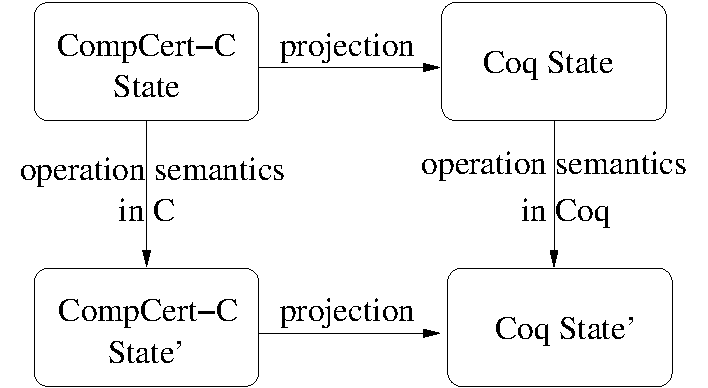
\includegraphics[width=.5\linewidth]{theorem.pdf}
\caption{Correctness of the simulation of an ARM operation}
\label{fig:thrm}
\end{figure}

In detail,
changes in the C memory model are formally described
by a transition system according to the operational semantics of Compcert-C.
Therefore, the later is used everywhere in the proofs. 
This operational semantics is described by
a big mutual inductive type;
in particular, the evaluation of expressions is defined by
16 constructors, one for each CompCert C expression such as assignment or binary
operation.
% And this inductive type evaluation of expression is our target to try the
% improved new inversion.
A typical proof step starts from a goal intuitively saying that,
given two C memory states related by a C expression,
as expressed in some hypothesis $H$, 
some commutative diagram holds.
Then $H$ is inverted, which either yields more elementary 
transitions between C memory states, 
with corresponding expected commutative diagrams,
or solves the current diagram if the considered expression
is atomic. 
In general we see that an inversion will result in many
new opportunities to perform inversions.

In our first proofs, using the Coq standard \inversion tactic
resulted in a very weak control on the script.
Finding the right relation to focus on in the hypotheses
was inconvenient.
Interactive execution of the script was also quite slow,
due to the size of the terms generated by \inversion.
And the compilation time for the proof on only one instruction 
took more than one minute --
there are more than one hundred instructions in the ARMv6 architecture.
Moreover
the proof code is fragile in case of changes: 
after \inversion, hypotheses are automatically given similar names 
according to a simple numbering scheme,
so that any modification at the beginning of the proof script
or in auxiliary lemmas 
result in a complete renaming of hypotheses to come in the sequel.
This is quite harmful in practice and constitutes
a serious issue for maintenance.

The following code shows an small excerpt from 
an old proof script in SimSoC-Cert using \inversion.
In this example, we want to find out the relation between memory states
\coqdocvar{m} and \coqdocvar{m'} expressed in the hypothesis $H$,
whose main argument (\coqdocvar{Ecall (Evalof...})
represents the program to be executed.
Its type is given by the inductive relation \coqdocvar{eval\_expr}.
%To achieve this goal, we use \inversion step
%following step by step the definition of semantics of \coqdocvar{eval\_expr}.
We see that many \coqdocvar{inv Hx} are used.
Here \coqdocvar{inv H} denotes \coqdocvar{inversion H; clear H; subst}.

\medskip
\dots \\
\coqdocinput{chunk41}

\coqdocinput{chunk42}
\dots
\medskip

The program for simulating an ARM instruction 
usually contains expressions more complex than in the
example given here.
% We have to invert the predicate so many times to find the relation between
% initial and final memory state. 
This cumbersome work is needed in correctness proofs for every instruction,
and there is no clear way to share anything since
the corresponding programs are rather specific,
at least for instructions belonging to different categories.

Thanks to the technique introduced in this paper,
we could define convenient reusable tactics.
First, we defined suitable diagonal-based functions for each
constructor of $eval\_expr$ following the lines given in the
previous section.
Then we packaged them together in a high-level tactic named 
$inv\_eval\_expr$ using an Ltac definition. The arguments of this
tactic are the memory states under focus --
in the example above: $m$ and $m'$.
This tactic also contains extra features so that
it is able to:
%
\begin{enumerate}
\item automatically find an hypothesis to be inverted;
\item repeatedly perform our hand-crafted inversion until all constraints
  between two memory states are derived;
\item give meaningful names to the derived constraints;
\item update all other related hypotheses according to the new 
  variable names or values;
\item clean up useless variables and hypotheses.
\end{enumerate}
%
Then all the eighteen \inversion in the example above are solved in just
one step using $inv\_eval\_expr~m~m'$.

To be fair, let us mention that the robustness issue could,
in principle, be managed using the current version of standard \inversion,
because it allows us 
to give explicit names to introduced variables and hypotheses.
However, due to the complexity of CompCert C semantics, 
providing all these names explicitly turns out to be cumbersome,
and unrealistic when you face dozens of consecutive \inversion 
and about ten names for each \inversion.
Within our framework,
the introduction of suitable names 
is automatically performed inside $inv\_eval\_expr m m'$.
Names are chosen according to the contents and in a flexible way, 
so that the evolution of goals is easy to follow.

As an unexpected benchmark, 
when CompCert C semantics has been changed to a new version
in the end of 2011,
we did not have to change the proofs:
just updating the tactic turned out to be enough. 

Comparing development times provides additional hints.
In our first try, dedicated to the instruction ADC,
more than two months were spent on the development of the correctness proof.
The inversion technique presented here was not available
at that time, entailing the drawbacks detailed above.
With the new approach, proofs for 4  other instructions
could be finished in only one week. 
The high-level tactic described above required
less than 2 weeks.


Finally, 
we compare the efficiency of the standard Coq \inversion with our new tactic
in Table.~\ref{t:timing}.
The first line is about the whole expression given in the example above. 
The other lines are inversions of specific expressions.
We can observe a gain of about 4 to 5 times.

\begin{table}\centering
\label{t:timing}
\caption{Comparison of the time costs}
\begin{tabular}{|l|c|c|}
\hline
 & standard \inversion & our inversion \\
\hline
Full example &  1.856& 0.404\\
\hline
Ebinop & 0.104&  0.020\\
\hline
Evalof &  0.096& 0.020\\
\hline
Eval &  0.116& 0.020\\
\hline
Evar &  0.108& 0.024\\
\hline
\end{tabular}
\end{table}



%%% Local Variables: 
%%% mode: latex
%%% TeX-master: "cpp12"
%%% End: 

\section{Conclusion}
\label{sec:conclusion}

The technique introduced in \cite{small_inv}
on very small toy examples
could be successfully used in a significant application,
up to suitable extensions in order to conveniently get
the premises of a constructor in non-absurd cases.
As in \cite{small_inv},
we don't claim that we have a fully automated tactic,
like \inversion.
Our goal is more modest:
providing a hand-crafted inversion technique 
which is flexible enough for the user,
so that most practical situations can be managed
with a full control on the script and valuable
improvements on robustness.
Moreover, the extra flexibility provided by hand-crafted inversions can
be exploited to produce smaller, more manageable proof terms.

Our method was experimented on large proofs relying on 
big inductive relations independently defined in the Compcert project.

The current development can be found on-line\footnote{%
\label{f:site}
%\url{http://formes.asia/media/simsoc-cert/}}
\url{http://www-verimag.imag.fr/~monin/Proof/SmallInvScalesUp/}
}.

Our group recently started another project dedicated
to a certifying compiler from a high-level component-based language dedicated
to embedded systems (BIP), with CompCert C as its target. 
We expect the work presented here and our high-level tactics
to be reused there.

Let us mention another possible application of the technique.
Inversion is sometimes
needed to write a function whose properties will be established later (as
opposed to providing a monolithic and exhaustive Hoare-style specification and
along with a VCC generator such as Program). 
In this context simply using the proof engine and the \inversion tactic
tends to generate unmanageably large terms.
We can expect our technique could be very helpful in such situations.


% and the line-count metrics given at the end of \cite{small_inv} makes sense



%%% Local Variables: 
%%% mode: latex
%%% TeX-master: "cpp12"
%%% End: 



\bibliographystyle{abbrv}
\bibliography{biblio}

\end{document}


%-------------------------------------------------------------------------


%%% Local Variables: 
%%% mode: latex
%%% TeX-master: "cpp12"
%%% End: 
